\documentclass[a4paper,11pt]{article}
\usepackage[utf8]{inputenc}
\usepackage[T1]{fontenc}
\usepackage[swedish]{babel}
\usepackage{amsmath,amssymb,amsfonts}
\usepackage{tikz}
\usepackage{enumitem}
\usepackage{geometry}
\usepackage{graphicx}
\usepackage{booktabs}
\usepackage{array}
\usepackage{xcolor}
\usepackage{float}
\geometry{margin=2.5cm}

\title{Evolutionens bevis - Upptäckarövning}
\author{Partille Gymnasium}
\date{\today}

\begin{document}

\maketitle

\begin{center}
\fbox{\parbox{0.93\textwidth}{
\textbf{Instruktioner:}\\
\vspace{2mm}
Studera bilderna noggrant och svara på frågorna. Du behöver INTE ha förkunskaper - använd bara dina observationer och logiskt tänkande.
\vspace{2mm}
}}
\end{center}

\newpage

\section{Del 1: Mystiska likheter}

\subsection{Uppgift A: Vad ser du?}

Studera bilderna av skelettstrukturer från olika djur:

\begin{figure}[H]
\centering
% PLACEHOLDER: Insert comparative bone structure images here
% Suggested images: Human arm, bat wing, whale flipper, bird wing bones
% Source: Natural History Museum, Smithsonian, or educational anatomy sites
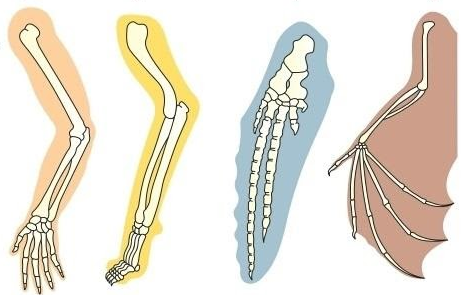
\includegraphics[width=0.8\textwidth]{homologous-organs.png}
\caption{Skelettstrukturer från fyra olika djur}
\end{figure}

\textbf{Observationer:}
\begin{enumerate}
    \item Vilka likheter ser du mellan dessa strukturer?
    
    \vspace{2.5cm}
    
    \item Vilka skillnader finns det?
    
    \vspace{2.5cm}
    
    \item Vilka typer av djur tror du strukturerna tillhör och vad har de för funktion?
    
    \vspace{2.5cm}
    \item Varför tror du strukturerna liknar varandra?
\end{enumerate}


\newpage
\subsection{Uppgift B: Färgkoda likheterna}

Rita av strukturerna och använd samma färg för ben som verkar motsvara varandra:
\begin{itemize}
    \item \textcolor{red}{\textbf{Röd}} för det längsta benet
    \item \textcolor{blue}{\textbf{Blå}} för de två mellanbenen  
    \item \textcolor{green}{\textbf{Grön}} för de små benen
    \item \textcolor{orange}{\textbf{Orange}} för ``fingrarna''
\end{itemize}

\newpage

\section{Del 2: Onödiga delar?}

\subsection{Uppgift C: Konstiga strukturer}

Studera dessa bilder av djur med ``konstiga'' kroppsdelar:

\begin{figure}[H]
\centering
\begin{tabular}{cc}
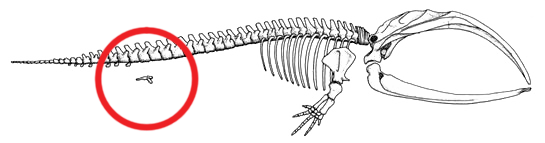
\includegraphics[width=0.4\textwidth]{whale_pelvis.png} & 
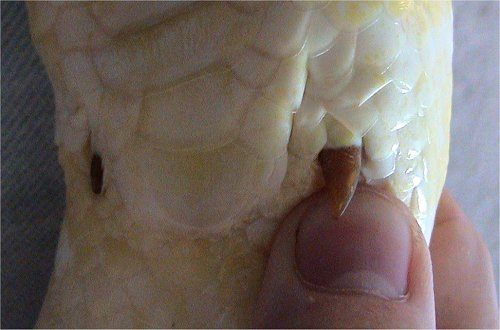
\includegraphics[width=0.4\textwidth]{Anal_spurs.jpg} \\
Valens bäckenben & Ormarnas bakben \\[0.5cm]
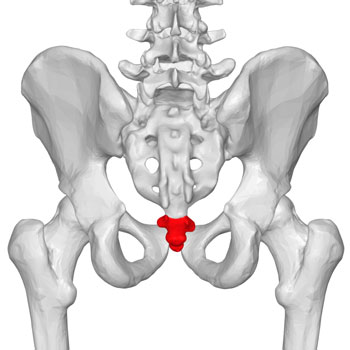
\includegraphics[width=0.4\textwidth]{human-coccyx.jpg} & 
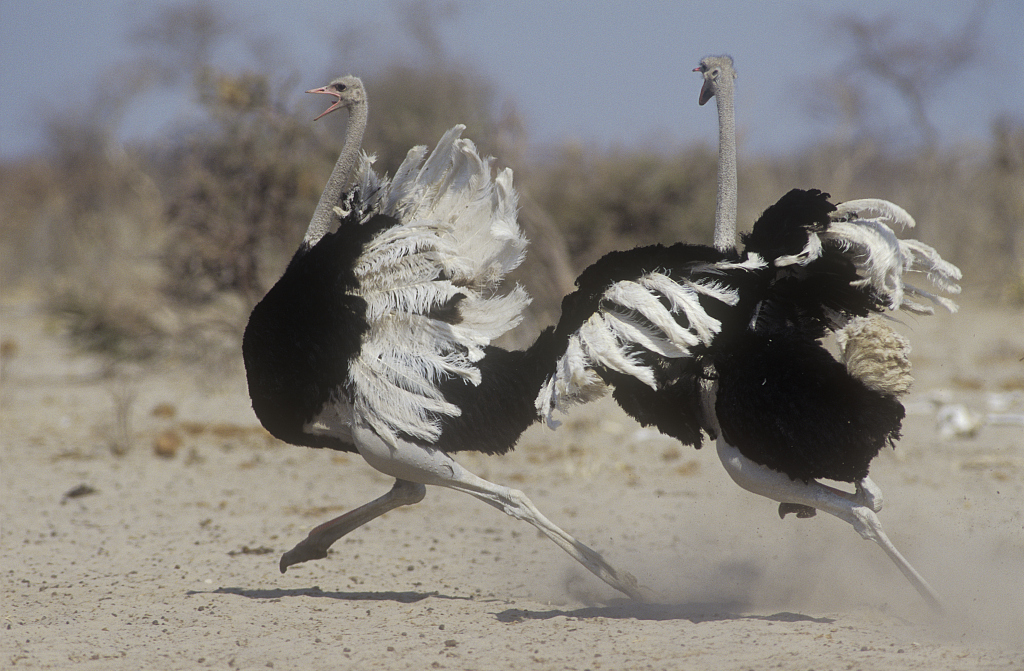
\includegraphics[width=0.4\textwidth]{ostrichrunning.jpeg} \\
Människans svankotor & Strutsfågelns vingar \\
\end{tabular}
\caption{Märkliga strukturer hos olika djur}
\end{figure}
\begin{enumerate}
    \item Vad är konstigt med dessa strukturer?
    
    \vspace{2cm}
    
    \item Varför tror du att djuren har dessa ``onödiga'' delar?
    
    \vspace{2cm}
    
    \item Kan du hitta liknande ``onödiga'' strukturer på din egen kropp? (Tips: känn längst ner på ryggraden, titta på dina visdomständer)
    
    \vspace{2cm}
\end{enumerate}

\section{Del 3: Embryonmysteriet}

\subsection{Uppgift D: Gissa djuret}

Titta på dessa bilder av mycket unga embryon (ofödda djur):

\begin{figure}[H]
\centering
% PLACEHOLDER: Insert early embryo comparison images here
% Suggested images: Fish, bird, mammal, human embryos at similar early stages
% Source: Developmental biology textbooks, educational sites (ensure accuracy)
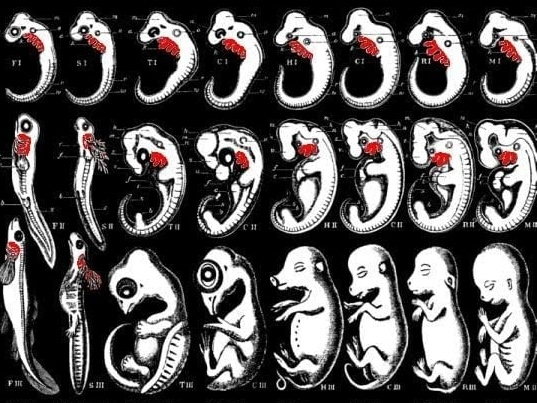
\includegraphics[width=0.8\textwidth]{embryo-drawings.jpg}
\caption{Embryon från åtta olika djurarter}
\end{figure}
\begin{enumerate}
    \item Kan du gissa vilka djur dessa embryon kommer från?
    
    \vspace{2cm}
    
    \item Vad ser du för likheter?
    
    \vspace{2cm}
    
    \item Alla har ``spalter'' (rött på bilden) på sidorna av huvudet. Vad tror du dessa blir hos olika djur?
    
    \vspace{2cm}
    
    \item Alla har en ``svans''. Vad händer med den hos olika djur?
\end{enumerate}

\newpage
\section{Del 4: Dina egna teorier}

\subsection{Uppgift F: Förklara mönstren}

Baserat på alla bilder du sett, försök förklara:

\begin{enumerate}
    \item Varför ser skelett från olika djur så lika ut?
    
    \vspace{2cm}
    
    \item Varför har djur ``onödiga'' kroppsdelar?
    
    \vspace{2cm}
    
    \item Varför ser embryon från olika djur så lika ut i början?
    
    \vspace{2cm}
    
    \item Kan du komma på EN förklaring som skulle kunna förklara ALLA dessa mönster?
    
    \vspace{3cm}
\end{enumerate}


\end{document}
